

\tikzset{every picture/.style={line width=0.75pt}} %set default line width to 0.75pt        

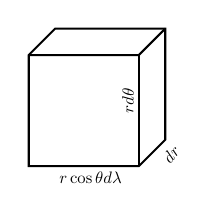
\begin{tikzpicture}[x=0.3pt,y=0.3pt,yscale=-1,xscale=1]
%uncomment if require: \path (0,300); %set diagram left start at 0, and has height of 300

%Shape: Cube [id:dp6183555325574622] 
\draw   (100,86.51) -- (131.71,54.8) -- (264.42,54.8) -- (264.42,188.56) -- (232.71,220.27) -- (100,220.27) -- cycle ; \draw   (264.42,54.8) -- (232.71,86.51) -- (100,86.51) ; \draw   (232.71,86.51) -- (232.71,220.27) ;

% Text Node
\draw (134.69,225.2) node [anchor=north west][inner sep=0.75pt]  [xscale=0.6,yscale=0.6]  {$r\cos \theta d\lambda $};
% Text Node
\draw (248.02,214.64) node [anchor=north west][inner sep=0.75pt]  [rotate=-311.53,xscale=0.6,yscale=0.6]  {$ \begin{array}{l}
dr\\
\end{array}$};
% Text Node
\draw (209.96,158.75) node [anchor=north west][inner sep=0.75pt]  [rotate=-271.45,xscale=0.6,yscale=0.6]  {$rd\theta $};


\end{tikzpicture}